\documentclass[aspectratio=43]{beamer}
\usepackage[spanish]{babel}
\selectlanguage{spanish}
\usepackage{amsthm}
\usepackage{amsfonts}
\usepackage{amsmath}
\usepackage{amssymb}
\usepackage{mathtools}
\usepackage{bbm}
\usepackage{pgfplots}
\usepackage{tikz}
\usepackage{physics}
\usepackage{calligra}
\usepackage{csquotes}
\usepackage{tensor}
\usepackage[thicklines]{cancel}
\usepackage{tcolorbox}
\usepackage{pstricks}
\pgfplotsset{compat=1.16}
% \usepackage{algorithm2e}
% \usepackage{algorithmic}
\usepackage{comment}
\usepackage{algpseudocode}
\usepackage{algorithm}
\makeatletter
\renewcommand{\ALG@name}{Algoritmo}
\makeatother

\usepackage{float}
\usepackage[backend=biber, style=apa]{biblatex} %Custom bibliography
    \addbibresource{ref.bib} %Load references


\DeclareMathAlphabet{\mathcalligra}{T1}{calligra}{m}{n}
\DeclareFontShape{T1}{calligra}{m}{n}{<->s*[2.2]callig15}{}
\newcommand{\scriptr}{\mathcalligra{r}\,}
\newcommand{\boldscriptr}{\pmb{\mathcalligra{r}}\,}
\def\rc{\scriptr}
\def\brc{\boldscriptr}
\def\hrc{\hat\brc}
\newcommand{\ie}{\emph{i.e.}} %id est
\newcommand{\eg}{\emph{e.g.}} %exempli gratia
\newcommand{\rtd}[1]{\ensuremath{\left\lfloor #1 \right\rfloor}}
\newcommand{\dirac}[1]{\ensuremath{\delta \left( #1 \right)}}
\newcommand{\diract}[1]{\ensuremath{\delta^3 \left( #1 \right)}}
\newcommand{\e}{\ensuremath{\epsilon_0}}
\newcommand{\m}{\ensuremath{\mu_0}}
\newcommand{\V}{\ensuremath{\mathcal{V}}}
\newcommand{\prnt}[1]{\ensuremath{\left(#1\right)}} %parentheses
\newcommand{\colch}[1]{\ensuremath{\left[#1\right]}} %square brackets
\newcommand{\chave}[1]{\ensuremath{\left\{#1\right\}}}  %curly brackets
\newcommand\eqdef{\stackrel{\mathclap{\normalfont \tiny\mbox{\textrm{def}}}}{=}}
\useoutertheme{infolines}
\useinnertheme{rectangles}
\usefonttheme{professionalfonts}


\definecolor{blue2}{HTML}{045FB4}
\definecolor{green2}{HTML}{46C235}
\definecolor{red2}{HTML}{EE4848}
\definecolor{violet2}{HTML}{A647E5}
\definecolor{orange2}{HTML}{FF7425}
\definecolor{darkred}{HTML}{5C2020}
\definecolor{gray}{HTML}{303030}
\definecolor{yellow}{HTML}{f0be52}
\definecolor{lightdarkgold}{HTML}{EEBC1D}

\renewcommand{\CancelColor}{\color{darkred}}

\makeatletter
\newcommand{\mybox}[1]{%
  \setbox0=\hbox{#1}%
  \setlength{\@tempdima}{\dimexpr\wd0+13pt}%
  \begin{tcolorbox}[colback=darkred,colframe=darkred,boxrule=0.5pt,arc=4pt,
      left=6pt,right=6pt,top=6pt,bottom=6pt,boxsep=0pt,width=\@tempdima]
    \textcolor{yellow}{#1}
  \end{tcolorbox}
}
\makeatother


\pgfplotsset{my style/.append style={axis x line=middle, axis y line=
middle, xlabel={$x$}, ylabel={$y$}, axis equal }}


\usecolortheme[named=darkred]{structure}
\usecolortheme{sidebartab}
\usecolortheme{orchid}
\usecolortheme{whale}
\setbeamercolor{titlelike}{parent=structure, bg=structure, fg=white}
\setbeamercolor{section in toc}{fg= white}
\setbeamercolor{subsection in toc}{fg= white}
%\setbeamercolor*{sidebar}{fg=red2,bg=gray!15!white}

\setbeamercolor{item projected}{bg=yellow, fg = darkred}
\setbeamertemplate{enumerate items}[default]
\setbeamertemplate{navigation symbols}{}
\setbeamercolor{local structure}{fg=yellow}

\setbeamercolor{alerted text}{fg=white}
\setbeamercolor{block title}{bg = blue2}
\setbeamercolor{block title alerted}{bg=red2}
\setbeamercolor{block title example}{bg=green2}
\setbeamercolor{background canvas}{bg=gray}
\setbeamercolor{normal text}{bg=gray,fg=white}


% this is to change the color in the bibliography, necessary because normal red cannot be normally red by this beamer
\setbeamercolor{bibliography item}{fg=white}
\setbeamercolor{bibliography entry author}{fg=yellow}
\setbeamercolor{bibliography entry title}{fg=white}
\setbeamercolor{bibliography entry location}{fg=white}
\setbeamercolor{bibliography entry note}{fg=white}


\setbeamertemplate{footline}
        {
      \leavevmode%
      \hbox{%
      \begin{beamercolorbox}[wd=.333333\paperwidth,ht=2.25ex,dp=1ex,center]{author in head/foot}%
        \usebeamerfont{author in head/foot}\insertshortauthor~~(\insertshortinstitute)
      \end{beamercolorbox}%
      \begin{beamercolorbox}[wd=.333333\paperwidth,ht=2.25ex,dp=1ex,center]{title in head/foot}%
        \usebeamerfont{title in head/foot}\insertshorttitle
      \end{beamercolorbox}%
      \begin{beamercolorbox}[wd=.333333\paperwidth,ht=2.25ex,dp=1ex,center]{date in head/foot}%
        \usebeamerfont{date in head/foot}\insertshortdate{}%\hspace*{2em}

    %#turning the next line into a comment, erases the frame numbers
        %\insertframenumber{} / \inserttotalframenumber\hspace*{2ex} 

      \end{beamercolorbox}}%
      \vskip0pt%
    }


\setbeamertemplate{blocks}[rectangle]
\setbeamercovered{dynamic}




%\setbeamercolor{author}{fg=yellow}
%\setbeamercolor{title}{fg = yellow}
%\setbeamerfont{title}{size=\Large, series=\bfseries}
%\setbeamerfont{author}{size=\footnotesize}
%\setbeamerfont{date}{size=\small}


\setbeamertemplate{section page}
{
	\begin{centering}
		\begin{beamercolorbox}[sep=27pt,center]{part title}
			\usebeamerfont{section title}\insertsection\par
			\usebeamerfont{subsection title}\insertsubsection\par
		\end{beamercolorbox}
	\end{centering}
}





%\setbeamertemplate{subsection page}
%{
%	\begin{centering}
%		\begin{beamercolorbox}[sep=12pt,center]{part title}
%			\usebeamerfont{subsection title}\insertsubsection\par
%		\end{beamercolorbox}
%	\end{centering}
%}

\newcommand{\hlight}[1]{\colorbox{violet!50}{#1}}
\newcommand{\hlighta}[1]{\colorbox{darkred!50}{#1}}

\title{EIF203 Quiz Kruskal} %->->->->-> Check hyperref title <-<-<-<-<-
\subtitle{Análisis del algoritmo de Kruskal}
\author[D. Quirós Artiñano]{\textcolor{yellow}{Diego Quirós Artiñano}\\ \small ID:901150326}
\institute[UNA]{
    \textcolor{white}{EIF-203: Estructuras Discretas NRC: 41712}%
    \\%
    \textcolor{white}{Universidad Nacional de Costa Rica}%
} %You can change the Institution if you are from somewhere else
\date{13 de junio, 2022}
\logo{
\includegraphics[width= 0.08\textwidth]{../../../UNAImage/UNA.png}}

\begin{document}
    
    \frame{\titlepage}

    \begin{frame}{Declaración Jurada}
        \textit{Declaro de manera jurada que este trabajo fue elaborado por mi persona de manera estrictamente individual y que las fuentes usadas son la declaradas en la lámina de referencias, las cuales sirvieron de base pero no fueron usadas como copia literal.}
    \end{frame}

    \section*{References} %You can remove this if you do not want to use it
        \begin{frame}[allowframebreaks]{Referencias}
            \printbibliography
        \end{frame}
    
    \begin{frame}{Tabla de Contenidos}
        \tableofcontents
    \end{frame}

    \section{Definiciones y explicaciones}
\frame{\sectionpage}

\begin{frame}{Minimum Spanning Tree o árbol de exploración mínimo}
    \begin{block}{Spanning Tree} % azul
        Según \cite{Goodaire_Parmenter_2001}, es un subgrafo de un grafo conectado que incluye todos los vertices
    \end{block}
    \begin{exampleblock}{Minimum Spanning Tree} %verde
        Es un subgrafo de un grafo con peso, pero con el mínimo peso posible
    \end{exampleblock}

    % alertblock es rojo, theorem es como block pero en indenta y demostration es igual que block
\end{frame}

\begin{frame}{Heurístico y Greedy}
    \begin{columns}
        \begin{column}{0.5\textwidth}
            \textcolor{yellow}{Algoritmo Heurístico:} Como visto en clase el algoritmo heurístico es el algoritmo que va haciendo decisiones sin conocimiento de lo siguiente. O como dicen en este foro (\cite{heuri}), es "Las heurísticas implican utilizar un enfoque de aprendizaje y descubrimiento para alcanzar una solución"
        \end{column}
        \begin{column}{0.5\textwidth}
            \textcolor{yellow}{Algoritmo Greedy:} Como se vio en clase el algoritmo greedy es un algoritmo heurístico que no hace backtracking.
            \begin{block}{Algoritmo de Kruskal}
                El algoritmo de Kruskal es un algoritmo heurístico y greedy para buscar el árbol de exploración de peso mínimo
            \end{block}
        \end{column}
    \end{columns}
\end{frame}

    \input{chapters/kruskalAlgorithm}
    \section{Ejemplos}
\frame{\sectionpage}

\begin{frame}{Ejemplo 1 (Clase 6 de junio)}
    \usetikzlibrary{arrows,shapes}
    
    \pgfdeclarelayer{background}
    \pgfsetlayers{background,main}
    
    \tikzstyle{vertex}=[circle,fill=black,minimum size=20pt,inner sep=0pt]
    \tikzstyle{selected vertex} = [vertex, fill=red]
    \tikzstyle{edge} = [draw,thick,-]
    \tikzstyle{weight} = [font=\small, color=yellow]
    \tikzstyle{selected edge} = [draw,line width=5pt,-,red!50]
    \tikzstyle{ignored edge} = [draw,line width=5pt,-,black!20]

    \begin{figure}
        \begin{tikzpicture}[scale=1.8, auto,swap]
            % Draw a 7,11 network
            % First we draw the vertices
            \foreach \pos/\name in {{(0,2)/a}, {(-1,1)/b}, {(-1,-1)/c},
                                    {(1,-1)/d}, {(1,1)/e}}
                \node[vertex] (\name) at \pos {$\name$};
            % Connect vertices with edges and draw weights
            \foreach \source/ \dest /\weight in {a/b/10, b/c/50, e/a/100, d/a/30, c/e/10, c/d/20, d/e/60}
                \path[edge] (\source) -- node[weight] {$\weight$} (\dest);
            % Start animating the vertex and edge selection. 
            \foreach \vertex / \fr in {a/1,b/2,c/3,e/4,d/5}
                \path<\fr-> node[selected vertex] at (\vertex) {$\vertex$};
            % For convenience we use a background layer to highlight edges
            % This way we don't have to worry about the highlighting covering
            % weight labels. 
            \begin{pgfonlayer}{background}
                \pause
                \foreach \source / \dest in {a/b,b/a,c/e,c/d,a/d}
                    \path<+->[selected edge] (\source.center) -- (\dest.center);
                \foreach \source / \dest / \fr in {b/c/7, d/e/8, e/a/9}
                    \path<\fr->[ignored edge] (\source.center) -- (\dest.center);
            \end{pgfonlayer}
        \end{tikzpicture}
    \end{figure}
\end{frame}

\begin{frame}{Resultado Ejemplo 1}
    \usetikzlibrary{arrows,shapes}
    
    \pgfdeclarelayer{background}
    \pgfsetlayers{background,main}
    
    \tikzstyle{vertex}=[circle,fill=black,minimum size=20pt,inner sep=0pt]
    \tikzstyle{selected vertex} = [vertex, fill=red]
    \tikzstyle{edge} = [draw,thick,-]
    \tikzstyle{weight} = [font=\small, color=yellow]
    \tikzstyle{selected edge} = [draw,line width=5pt,-,red!50]
    \tikzstyle{ignored edge} = [draw,line width=5pt,-,black!20]
    
    \begin{figure}
        \begin{tikzpicture}[scale=1.8, auto, swap]
            \foreach \pos/\name in {{(0,2)/a}, {(-1,1)/b}, {(0,0)/c},
                                    {(1,1)/d}, {(0,-1)/e}}
                \node[vertex] (\name) at \pos {$\name$};
            \foreach \source/ \dest /\weight in {a/b/10, d/a/30, c/e/10, c/d/20}
                \path[edge] (\source) -- node[weight] {$\weight$} (\dest);
        \end{tikzpicture}
    \end{figure}

    Peso del árbol: 70
\end{frame}

\begin{frame}{Ejemplo 2 (Ejercicio 6, Práctica Parcial 2)}
    \usetikzlibrary{arrows,shapes}
    
    \pgfdeclarelayer{background}
    \pgfsetlayers{background,main}
    
    \tikzstyle{vertex}=[circle,fill=black,minimum size=20pt,inner sep=0pt]
    \tikzstyle{selected vertex} = [vertex, fill=red]
    \tikzstyle{edge} = [draw,thick,-]
    \tikzstyle{weight} = [font=\small, color=yellow]
    \tikzstyle{selected edge} = [draw,line width=5pt,-,red!50]
    \tikzstyle{ignored edge} = [draw,line width=5pt,-,black!20]

    \begin{figure}
        \begin{tikzpicture}[scale=1.8, auto,swap]
            % Draw a 7,11 network
            % First we draw the vertices
            \foreach \pos/\name in {{(0,0)/a}, {(1,1)/b}, {(1,0)/c},
                                    {(1,-1)/d}, {(2,0)/e}, {(3,1)/f}, {(3,-1)/g}}
                \node[vertex] (\name) at \pos {$\name$};
            % Connect vertices with edges and draw weights
            \foreach \source/ \dest /\weight in {b/a/4, c/a/9, a/d/3, c/b/5, f/b/7, d/c/1, e/c/6, d/e/2, d/g/4, f/e/8, e/g/7, f/g/2}
                \path[edge] (\source) -- node[weight] {$\weight$} (\dest);
            % Start animating the vertex and edge selection. 
            \foreach \vertex / \fr in {c/1, d/2, e/3, f/4, g/5, a/6, b/7}
                \path<\fr-> node[selected vertex] at (\vertex) {$\vertex$};
            % For convenience we use a background layer to highlight edges
            % This way we don't have to worry about the highlighting covering
            % weight labels. 
            \begin{pgfonlayer}{background}
                \pause
                \foreach \source / \dest in {c/d, d/e, e/d, f/g, a/d, a/b, d/g}
                    \path<+->[selected edge] (\source.center) -- (\dest.center);
                \foreach \source / \dest / \fr in {b/c/8, c/e/9, b/f/10, e/g/10, e/f/11, a/c/12}
                    \path<\fr->[ignored edge] (\source.center) -- (\dest.center);
            \end{pgfonlayer}
        \end{tikzpicture}
    \end{figure}
\end{frame}

\begin{frame}{Resultado Ejemplo 2}
    \usetikzlibrary{arrows,shapes}
    
    \pgfdeclarelayer{background}
    \pgfsetlayers{background,main}
    
    \tikzstyle{vertex}=[circle,fill=black,minimum size=20pt,inner sep=0pt]
    \tikzstyle{selected vertex} = [vertex, fill=red]
    \tikzstyle{edge} = [draw,thick,-]
    \tikzstyle{weight} = [font=\small, color=yellow]
    \tikzstyle{selected edge} = [draw,line width=5pt,-,red!50]
    \tikzstyle{ignored edge} = [draw,line width=5pt,-,black!20]
    
    \begin{figure}
        \begin{tikzpicture}[scale=1.8, auto, swap]
            \foreach \pos/\name in {{(0,2)/d}, {(-2,1)/a}, {(-1,1)/c},
                                    {(1,1)/e}, {(2,1)/g}, {(-2,0)/b}, {(2,0)/f}}
                \node[vertex] (\name) at \pos {$\name$};
            \foreach \source/ \dest /\weight in {d/a/3, c/d/1, d/e/2, g/d/4, a/b/4, g/f/2}
                \path[edge] (\source) -- node[weight] {$\weight$} (\dest);
        \end{tikzpicture}
    \end{figure}

    Peso del árbol: 16
\end{frame}

    % \section{Blocks and Colors}
 \frame{\sectionpage}

\begin{frame}{Color}

    Just testing something don't mind this piece of code : \cite{cervantes1999}
\begin{itemize}
    \item \textcolor{blue2}{That's the blue2 color}
    \item \textcolor{green2}{That's the green2 color}
    \item \textcolor{red2}{That's the red2 color}
    \item \textcolor{violet2}{That's the violet2 color}
    \item \textcolor{orange2}{That's the orange2 color}
    \item \textcolor{yellow}{That's the yellow color}
\end{itemize}
    
\end{frame}

\begin{frame}{Blocks}
\begin{block}{begin block}
There's a block
\end{block}

\begin{alertblock}{begin alertblock}
    there's a alert block 
\end{alertblock}

\begin{exampleblock}{begin example block}
here comes example
\end{exampleblock} 

\end{frame}


\begin{frame}{Blocks}
    
\begin{theorem}
    Here comes a theorem
\end{theorem}

\begin{proof}
    Here comes the proof
\end{proof}


    
\end{frame}
    
    % \section{boxes and columns}
 \frame{\sectionpage}
 
\begin{frame}{Box}
    \begin{center}
        \textcolor{yellow}{\fbox{phrase inside box}} 

    \bigskip    
    
    \fbox{\parbox{\textwidth}{A big box\\ \[ 
    \{R^n_{\alpha}(0) \; | \; n \in \mathbb{N}\} = \{n\alpha \; \mathrm{mod}\;1 \; | \; n \in \mathbb{N}\} \]
    é denso em \([0,1)\). }}
 \end{center}
\end{frame}
    
\begin{frame}{Two Columns entire page}
\small

\begin{columns}
\begin{column}{0.5\textwidth}
\tiny \pause \textcolor{yellow}{Obs:} \(\alpha \eqdef \log b \in \mathbb{R}\backslash\mathbb{Q}\)
\small \pause 
   \begin{align*}
    R_\alpha \colon [0,1) &\longrightarrow [0,1) \\
                      x   &\longmapsto x + \alpha \; \mathrm{mod}\;1           
\end{align*}
\pause 
\small 
Here we can write some text Here we can write some text Here we can write some text Here we can write some text Here we can write some text  Here we can write some text  Here we can write some text
\end{column}
\begin{column}{0.5\textwidth}  %%<--- here
\pause 
\[R^n_\alpha(x) \eqdef R_\alpha \overbrace{\circ \ldots \circ }^{n} R_\alpha(x)\]

\pause 

Here we can write some text Here we can write some text Here we can write some text Here we can write some text Here we can write some text  Here we can write some text  Here we can write some text

\bigskip 

\footnotesize 
\textcolor{yellow}{\fbox{\parbox{\textwidth}{Question??????????? tell me if you want}}} 
\bigskip

the answer is 
\pause 
\textcolor{green2}{YES!!!!} \textcolor{green2}{because that that and that} or..

\bigskip 

The answer is \textcolor{red2}{NO!!!!} \textcolor{red2}{because that that and that}

\end{column}
\end{columns}

\end{frame}
    
    
\begin{frame}{Table and minipage}

\begin{center}
\begin{tabular}{|l|l|l|l|l|l|l|l|l|l|l|l|l|}
\hline
\(n\) & 1  & 2 & 3 & 4 & 5 & 6 & 7 & 8 & 9 & 10 & 11 & \ldots       \\ \hline
\(2^n\) & \textcolor{yellow}{2} & \textcolor{yellow}{4} & \textcolor{yellow}{8} & \textcolor{yellow}{1}6 & \textcolor{yellow}{3}2 & \textcolor{yellow}{6}4 & \textcolor{yellow}{1}28 &  \textcolor{yellow}{2}56 & \textcolor{yellow}{5}12 & \textcolor{yellow}{1}024 & \textcolor{yellow}{2}048 & \ldots    \\ \hline
\end{tabular}
\end{center}

\pause 

\bigskip

\begin{center}
\textcolor{yellow}{\fbox{o dígito 1 é mais frequente que o dígito 3?}}
\bigskip

\pause \tiny Spoiler: \textcolor{green2}{YES}.

\end{center}


\pause 
\bigskip
\small 
\
\pause 
\begin{minipage}{0.47\textwidth}
    Um conjunto de números satisfaz a \emph{\textcolor{yellow}{lei de Benford}} se o primeiro dígito \(d \in \{1,2,3,4,5,6,7,8,9\} \) ocorre com a seguinte proporção 
\end{minipage}
\begin{minipage}{0.47\textwidth}
    \centering  \textcolor{yellow}{\(P(d) = \log\bigg(1+ \frac{1}{d}\bigg) \)} 
\end{minipage}
\end{frame}

    
    % \section{Equations and Figure}
     
    \frame{\sectionpage}
    
    \begin{frame}{Ordinary Differential Equations}
        \uncover<+->{\begin{equation*}
            \dv{x} y(x) + \frac{1}{CR} y(x) = 0
        \end{equation*}}
        
        \uncover<+->{\begin{equation}
            \dv[2]{x} y(x) + \gamma \dv{x} y(x) + \omega_0^2 y(x) = f(x)
        \end{equation}}
    \end{frame}
    
    \begin{frame}{}
        \uncover<+>{\begin{equation*}
            \dv[2]{x} y(x) + \gamma \dv{x} y(x) + \omega_0^2 y(x) = f(x)
        \end{equation*}}
        \uncover<+>{\[ \Downarrow \]
        \begin{equation*}
            \colch{\dv[2]{x} + \gamma \dv{x} + \omega_0^2} y(x) = f(x)
        \end{equation*}}
        \uncover<+>{\[ \Downarrow \]
        \begin{equation*}
            y(x) = \frac{f(x)}{\dv[2]{x} + \gamma \dv{x} + \omega_0^2}
        \end{equation*}}
    \end{frame}
    
    \begin{frame}{Imagem}
        \centering
        %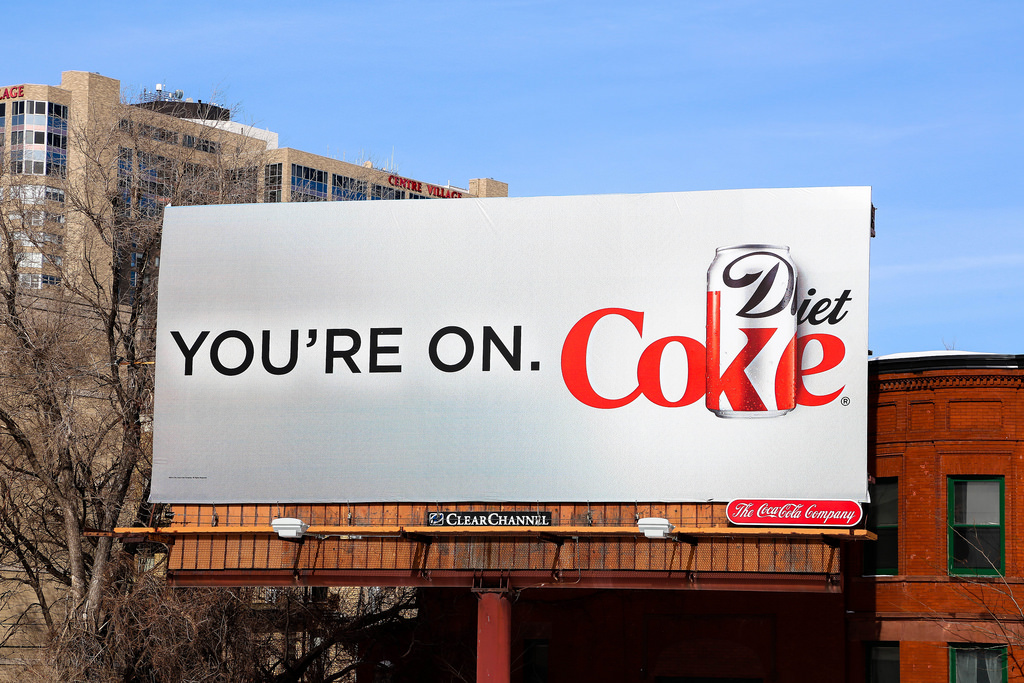
\includegraphics[width = 0.8\textwidth]{images/coke.jpg}\\
        \footnotesize \textcolor{yellow}{Figure:} Some words about the figure here
    \end{frame}
    
 
    \begin{frame}{See how is cool the fourier serie}
        \uncover<+>{\begin{equation*}
            \mathcal{F}[f](\xi) = \hat{f}(\xi) = \frac{1}{\sqrt{2\pi}} \int_{-\infty}^{+\infty} f(x) e^{-i x \xi} \dd{x}
        \end{equation*}}
        \uncover<+>{\begin{equation*}
            \mathcal{F}^{-1}[\hat{f}](x) = f(x) = \frac{1}{\sqrt{2\pi}} \int_{-\infty}^{+\infty} \hat{f}(\xi) e^{i x \xi} \dd{\xi}
        \end{equation*}}
    \end{frame}
    
    \begin{frame}{Quality Control}
        \uncover<+>{\begin{equation*}
            \widehat{(f + \alpha g)}(\xi) = \frac{1}{\sqrt{2\pi}} \int_{-\infty}^{+\infty} \prnt{f(x) + \alpha g(x)} e^{-i x \xi} \dd{x}
        \end{equation*}}
        \uncover<+>{\[ \Downarrow \]
        \begin{equation*}
            \widehat{(f + \alpha g)}(\xi) = \frac{1}{\sqrt{2\pi}} \int_{-\infty}^{+\infty} f(x) e^{-i x \xi} \dd{x} + \frac{\alpha}{\sqrt{2\pi}} \int_{-\infty}^{+\infty} g(x) e^{-i x \xi} \dd{x}
        \end{equation*}}
        \uncover<+>{\[ \Downarrow \]
        \begin{equation*}
            \widehat{(f + \alpha g)}(\xi) = \hat{f}(\xi) + \alpha \hat{g}(\xi)
        \end{equation*}}
    \end{frame}
    
    \begin{frame}{Quality Control}
        \uncover<+>{\begin{equation*}
            \widehat{f'}(\xi) = \frac{1}{\sqrt{2\pi}} \int_{-\infty}^{+\infty} f'(x) e^{-i x \xi} \dd{x}
        \end{equation*}}
        \uncover<+>{\[ \Downarrow \]
        \begin{equation*}
            \widehat{f'}(\xi) = \eval{\frac{f(x) e^{-ix\xi}}{\sqrt{2\pi}}}^{+\infty}_{-\infty} + i\xi \cdot \frac{1}{\sqrt{2\pi}} \int_{-\infty}^{+\infty} f(x) e^{-i x \xi} \dd{x}
        \end{equation*}}
        \uncover<+>{\[ \Downarrow \]
        \begin{equation*}
            \widehat{f'}(\xi) = i\xi \widehat{f}(\xi)
        \end{equation*}}
    \end{frame}
    
    \begin{frame}{Quality Control}
        \centering
        \textcolor{green2}{\huge{The inverse does work}}
        
        \normalsize{for appropriate functions} 
        
        \tiny{and, sometimes, the Fourier Transform of a function is not in the same set as the original function, but let's forget about this since we do not know a decent theory of integration}
    \end{frame} 
    
    % \section{graphs and other tikz}
 \frame{\sectionpage}
 
\begin{frame}{Drawning within tikz}
    \tikzset{every picture/.style={line width=0.75pt}} %set default line width to 0.75pt        

\begin{tikzpicture}[x=0.75pt,y=0.75pt,yscale=-1,xscale=1]
%uncomment if require: \path (0,486); %set diagram left start at 0, and has height of 486

%Curve Lines [id:da9595099437611456] 
\draw    (233.23,183.24) .. controls (252.87,215.34) and (288.86,227.45) .. (323.09,223.22) .. controls (353.65,219.45) and (382.81,202.65) .. (397.65,175.44) ;
%Curve Lines [id:da6932103982097759] 
\draw    (244.67,197.26) .. controls (301.86,150.51) and (339.03,156.74) .. (383.35,191.03) ;
%Curve Lines [id:da7053828945347995] 
\draw    (126,173.88) .. controls (131.72,222.2) and (184.62,311.04) .. (317.59,307.92) .. controls (450.55,304.8) and (507.74,212.85) .. (499.16,173.88) ;
%Curve Lines [id:da583602680611125] 
\draw    (126,173.88) .. controls (174.61,52.32) and (437.68,50.76) .. (499.16,173.88) ;
%Curve Lines [id:da5190289437371578] 
\draw [color={rgb, 255:red, 208; green, 2; blue, 27 }  ,draw opacity=1 ]   (126,173.88) .. controls (175,318) and (478,278) .. (499.16,173.88) ;
%Curve Lines [id:da5494113181101443] 
\draw [color={rgb, 255:red, 74; green, 144; blue, 226 }  ,draw opacity=1 ]   (313,222) .. controls (294,238) and (299,291) .. (317.59,307.92) ;
%Curve Lines [id:da8828117501564781] 
\draw [color={rgb, 255:red, 74; green, 144; blue, 226 }  ,draw opacity=1 ] [dash pattern={on 0.84pt off 2.51pt}]  (313,222) .. controls (330,233) and (336,298) .. (317.59,307.92) ;
%Shape: Parallelogram [id:dp02778297397005436] 
\draw  [fill={rgb, 255:red, 144; green, 144; blue, 144 }  ,fill opacity=0.44 ] (145.57,94) -- (308.5,94) -- (238.68,242.38) -- (75.75,242.38) -- cycle ;
%Shape: Circle [id:dp8371213746664339] 
\draw  [color={rgb, 255:red, 253; green, 1; blue, 1 }  ,draw opacity=1 ][fill={rgb, 255:red, 255; green, 0; blue, 0 }  ,fill opacity=1 ] (195.13,164.19) .. controls (195.13,163.08) and (196.02,162.19) .. (197.13,162.19) .. controls (198.23,162.19) and (199.13,163.08) .. (199.13,164.19) .. controls (199.13,165.29) and (198.23,166.19) .. (197.13,166.19) .. controls (196.02,166.19) and (195.13,165.29) .. (195.13,164.19) -- cycle ;
%Straight Lines [id:da21346648436809335] 
\draw [color={rgb, 255:red, 65; green, 117; blue, 5 }  ,draw opacity=1 ]   (197.13,164.19) -- (181.9,194.22) ;
\draw [shift={(181,196)}, rotate = 296.88] [color={rgb, 255:red, 65; green, 117; blue, 5 }  ,draw opacity=1 ][line width=0.75]    (10.93,-3.29) .. controls (6.95,-1.4) and (3.31,-0.3) .. (0,0) .. controls (3.31,0.3) and (6.95,1.4) .. (10.93,3.29)   ;

% Text Node
\draw (501,122.4) node [anchor=north west][inner sep=0.75pt]    {$\ $};
% Text Node
\draw (478,109) node [anchor=north west][inner sep=0.75pt]   [align=left] {\(\mathbb{T}\)};
% Text Node
\draw (82,65) node [anchor=north west][inner sep=0.75pt]   [align=left] {\(T_x\mathbb{T}\)};
% Text Node
\draw (206,152) node [anchor=north west][inner sep=0.75pt]   [align=left] {\textcolor{red2}{{\footnotesize \(x\)}}};
% Text Node
\draw (191.06,183.09) node [anchor=north west][inner sep=0.75pt]   [align=left] {{\footnotesize \textcolor{green2}{\(v\)}}};

\end{tikzpicture}

    
\end{frame}



\begin{frame}{It's possible plotting graphs with pgfplots and tikz}

\centering
\begin{tikzpicture}
\begin{axis}
\addplot[color=yellow]{exp(x)};
\end{axis}
\end{tikzpicture}
%Here ends the 2D plot

%Here ends the 3D plot

\end{frame}

\begin{frame}{Plotting 3d}
%Here begins the 3D plot
\centering
\begin{tikzpicture}
\begin{axis}
\addplot3[
    surf,
]
{exp(-x^2-y^2)*x};
\end{axis}
\end{tikzpicture}
\end{frame}

    % \section{}
    % \begin{frame}{}
    %     \centering
    %         \Huge\bfseries
    %     \textcolor{yellow}{The End}
    % \end{frame}
\end{document}
